\Section{Network Setup}

In this chapter the cINN setup which will be used for inferring the signal strength modifiers $\mu_i$ will be discussed. In the first half, the generation of the training and test datasets with a detailed focus on the analysis specifics, such as interpolation between histograms and the representation of the statistic and systematic uncertainties is going to be elaborated.

In the second half of this chapter, the final cINN architecture is going to be presented. The inference results and the interpretation of the network outputs will be discussed in the next chapter.

\Subsection{Training Dataset Generation}

The conditions shown in fig. \ref{fig:conditions} in chapter \ref{ch:analysis_strategy} represent the SM expectation. In order to infer the signal strength modifier parameters correctly, the network is trained on a dataset with varying signal strength and nuisance parameters. For this purpose, both signal and background processes have to be scaled to achieve the desired sensitivity towards different scenarios.

\Subsubsection{Prior Selection}

To construct the training dataset, a set of signal modifier parameters are drawn from a pool of expected parameter distributions, the prior distributions. Then, each process in the histogram is scaled with the corresponding parameter and the bins will summed up meaning the information about the exact contribution of each process to each bin is dropped.

The prior distribution for the processes have been selected as the following. For the signal processes \texttt{ggZH}, \texttt{ZHDY} and \texttt{WH} the $\mu_i$ were sampled from a gamma distribution

\begin{equation*}
	\Gamma(x; k, \theta) = \frac{x^{k-1}e^{-x/\theta}}{\theta^k\Gamma(k)}
\end{equation*}

with shape parameter $k$, scale $\theta$ and $\Gamma(k)$ being the gamma function. An advantage of this distribution as prior is the positiveness of the samples $\{x_i\}$ from the distribution as negative signal modifier parameters carry no physical meaning; apart from that, the distribution has a long tail for increasing values of $x$ which allow a more fined sampling around the SM expectation while maintaining some generalization property. The parameters were set to be $k = 1.5$ and $\theta = 7$; with this specific selection, one obtains a prior which is very sensitive in the low signal yield region $\mu \lesssim 10$ while maintaining network sensitivity for values $\mu\lesssim100$.

For the background processes, it is expected that the MC simulations follow the expectation with good accuracy. Hence, one expects $\mu \approx 1$. For this reason, the prior has been chosen to follow a lognormal distribution

\begin{equation*}
	\mathcal{N}(x; \mu, \sigma) = \frac{1}{\sqrt{2\pi }\sigma x}\exp\left(-\frac{\left(\ln x-\mu\right)^2}{2\sigma^2}\right)
\end{equation*}

with $\mu = 0.05$ and $\sigma = 0.25$, lognormal distributions being positive themselves. The resulting distribution has then a mean of 1.08 and standard deviation of 0.28.

In order the estimate the arising uncertainty from the luminosity, the obtained conditions (after scaling and uncertainty variation) are then scaled with an additional luminosity factor. These have been drawn from a lognormal distribution with $\mu = 0$ and $\sigma = 0.02$ and has a mean of 1.00 with standard deviation of 0.02. All distributions are shown in fig. \ref{fig:priors}.

With these priors, the cINN has a total of 17 inputs for 3 signal, 13 background modifier parameters and the luminosity nuisance parameter.

\begin{figure}[h!]
	\centering
	\includegraphics[width=\linewidth]{figures/network_setup/priors.pdf}
%	\begin{minipage}{.5\textwidth}
%		\centering
%%		\includegraphics[width=0.8\linewidth]{figures/network/signal}
%	\end{minipage}%
%	\begin{minipage}{.5\textwidth}
%		\centering
%%		\includegraphics[width=0.6\linewidth]{figures/network_setup/priors.pdf}
%	\end{minipage}
	\caption{Prior distributions for the signal and background processes. Samples are shown in blue; the mean of each distribution is shown with the red dashed line. The analytic shape of each distribution is shown in orange.}
	\label{fig:priors}
\end{figure}

In order to avoid that the network learns features not present in a general measured dataset the systematic effects have to be mapped onto the training and test dataset.

\Subsubsection{Systematic Uncertainties}

The systematic effects can be grouped into normalization and shape-changing effects.
Normalization uncertainties have an equal effect on each bin. To this group belong the following: the luminosity uncertainty and the background normalization uncertainty. Both the background modifier and the luminosity nuisance parameters represent these effects.

The shape-changing systematic uncertainties require an interpolation method as the shifts in the histograms are computationally expensive to obtain and are not available eihter. In other words, as only the effect of the $1\sigma$ up- and down-shifts of the uncertainties (templates) are given, the task is to interpolate between and to extrapolate from these histograms. For this purpose, a non-linear histogram morphing method has been implemented.

In the following, an overview on the considered uncertainties and the morphing algorithm will be given, followed by a discussion on the implementation and on its effects on the histograms.

\Subsubsection{Shape-Changing Uncertainties}

There are 25 nuisance parameter which have been taken into account. These can be grouped into normalization and shape-changing uncertainties.

The shape-changing uncertainties influence all histogram bins differently and incorporate most uncertainties in this setup. The shape-changing uncertainties have been listed in tab. \ref{tab:s_sys_table}. The interpolation among these systematic effects, given the $1\sigma$ shifted histograms, have been performed via histogram morphing, which will be discussed in the next section.

\begin{table}[h!]
	\centering
	\begin{tabular}{cc}
		Uncertainty name               & Description \\
		
		\hline
		\texttt{PDFSet} & Parton density function uncertainty \\
		
		\hline
		$\begin{aligned}
			\texttt{PSWeight}&\texttt{\_FSR} & \\
			\texttt{PSWeight}&\texttt{\_ISR} & \\
		\end{aligned}$ & $\begin{array}{c}
			\text{Parton shower modelling uncertainties} \\
			\text{for final and initial state radiation}
		\end{array}$ \\
		
		\hline
		$\begin{aligned}	
			\texttt{ScaleWeight}&\texttt{\_Envelope} \\
			\texttt{ScaleWeight}&\texttt{\_Fact    } \\
			\texttt{ScaleWeight}&\texttt{\_Mixed   } \\
			\texttt{ScaleWeight}&\texttt{\_Renorm  } \\
		\end{aligned}$ & Renormalization and factorization scale uncertainties \\
		
		\hline
		% https://twiki.cern.ch/twiki/bin/viewauth/CMS/BtagRecommendation#preUL_scale_factor_uncertainties
		$\begin{aligned}
			\texttt{btagWeight}&\texttt{\_lf       } \\
			\texttt{btagWeight}&\texttt{\_cferr1   } \\
			\texttt{btagWeight}&\texttt{\_cferr2   } \\
			\texttt{btagWeight}&\texttt{\_hf       } \\
			\texttt{btagWeight}&\texttt{\_hfstats1 } \\
			\texttt{btagWeight}&\texttt{\_hfstats2 } \\
			\texttt{btagWeight}&\texttt{\_lfstats1 } \\
			\texttt{btagWeight}&\texttt{\_lfstats2 } \\
		\end{aligned}$ & b-tagging correction uncertainties \\
		
		\hline
		\texttt{l1\_ecal\_prefiring  } & 2017 ECAL miss-calibration correction uncertainty \\
		
		\hline		
		% https://twiki.cern.ch/twiki/bin/view/CMS/MuonReferenceEffs2017
		$\begin{aligned}
			\texttt{electron}&\texttt{\_reco } \\
			\texttt{electron}&\texttt{\_id   } \\
			\texttt{muon}&\texttt{\_id       } \\
			\texttt{muon}&\texttt{\_iso      } \\
		\end{aligned}$         & $\begin{array}{c}
			\text{Lepton identification, reconstruction} \\
			\text{and isolation uncertainties}
		\end{array}$\\
		
		\hline
		$\begin{aligned}
			\texttt{trigger}&\texttt{\_ee\_sf  } \\
			\texttt{trigger}&\texttt{\_mu\_sf  } \\
			\texttt{trigger}&\texttt{\_mumu\_sf} \\
		\end{aligned}$ & Trigger efficiency uncertainties \\
		\hline
		% https://twiki.cern.ch/twiki/bin/view/CMS/PileupSystematicErrors
		\texttt{pileup               } & Pileup uncertainty \\
	\end{tabular}
	\caption{The shape-changing uncertainties with a brief description.}
	\label{tab:s_sys_table}
\end{table}

\Subsubsection{Non-Linear Histogram Morphing}

Non-linear histogram morphing has been implemented on the basis of \cite{Baak_2015}. For the interpolation a nominal distribution and -- in this case -- 24 additional distribution templates representing the $1\sigma$ and $-1\sigma$ shifts are given. The nominal template $f(x|m)$ with morphing parameter $m$ can then be approximated around $m=0$ with the other templates in a simple 1D case using

\begin{equation*}
	f(x|m) \approx \sum_j \left.\frac{\partial^{(j)} f(x|m)}{\partial m^{(j)}}\right|_{m=0}\frac{m^j}{j!} = \sum_j f_j'(x|m=0) m^j
\end{equation*}



where the derivatives and the factorials have been absorbed in $f'_j$.

For the $T$ uncorrelated uncertainties there are $T$ morphing parameters $m$ which take the values values $m\pm1$. In total, there are $2T+1$ sampled distributions with the nominal distribution with morphing parameter value $m=0$. An intuitive representation of the "morphing parameter space" with the indication of the available templates is shown in fig. \ref{fig:morphing_phase_space}. In the setting described above, one has $T=24$, hence there are $24\times2 +1 = 49$ templates in total.

\begin{figure}[h!]
	\centering
	\centering
	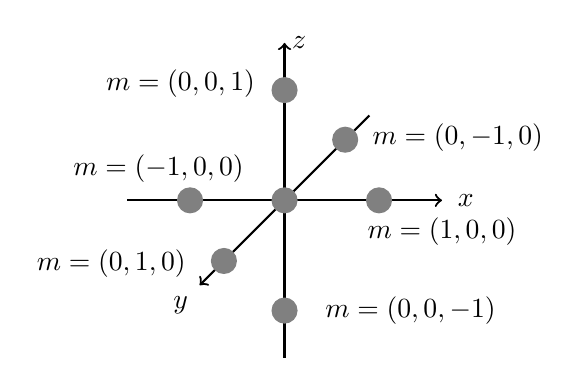
\begin{tikzpicture}[scale=2]
		\coordinate (O) at (0,0,0);
		\draw[thick,->] (-1.,0,0) -- (1.,0,0) node[right=2]{$x$};
		\draw[thick,->] (0,-1,0) -- (0,1,0) node[right=-1]{$z$};
		\draw[thick,->] (0,0,-1.4) -- (0,0,1.4) node[below left=0.5]{$y$};
		
		\node[circle, fill=gray] (0) {};
		\node[circle, fill=gray] at (   0,-0.7, 0) {};
		\node at (0.8, -0.7, 0) {$m=(0,0,-1)$};
		\node[circle, fill=gray] at (   0, 0.7, 0) {};
		\node at (-1.2, 0.2, -1.4) {$m=(0,0,1)$};
		\node[circle, fill=gray] at (   0, 0  ,-1) {};
		\node at (-0.8, 0.2, 0) {$m=(-1,0,0)$};
		\node[circle, fill=gray] at (   0, 0  , 1) {};
		\node at (1, -0.2, 0) {$m=(1,0,0)$};
		\node[circle, fill=gray] at (-0.6, 0  , 0) {};
		\node at (-1.1, -0.4, 0) {$m=(0,1,0)$};
		\node[circle, fill=gray] at ( 0.6, 0  , 0) {};
		\node at (1.1, 0.4, 0) {$m=(0,-1,0)$};
	\end{tikzpicture}
	\caption{The "morphing parameter space" showing the available distributions for $T=3$ uncertainties of $\sigma=\pm1$. The available templates in the phase space are shown in grey. Note that the nominal template with $m=(0,0,0)$ lies in the origin and there are no "mixed" templates (such as $m = (1,1,0)$) available.}
	\label{fig:morphing_phase_space}
\end{figure}

For this multidimensional case where there are no "mixed templates" as the above uncertainties are considered to be uncorrelated. Hence, the mixed derivative terms from the above expansion are zero and the expression can be written for a given $\mathbf{m}_i$\footnote{$\mathbf{m}_i = (0, 0, ..., 0, \pm 1, 0, ..., 0)$ for the i-th template with $\sigma=\pm1$} as:

\begin{equation}
	f(x | \mathbf{m}_i) = \underbrace{\vphantom{\frac{1}{2!}\left.\frac{\partial^2 f(x | \mathbf{m})}{\partial m_j^2}\right|_{\mathbf{m}=0}}f(x | 0)}_{f_0} + \sum^T_{j=1} \underbrace{\vphantom{\frac{1}{2!}\left.\frac{\partial^2 f(x | \mathbf{m})}{\partial m_j^2}\right|_{\mathbf{m}=0}}\left.\frac{\partial f(x | \mathbf{m})}{\partial m_j}\right|_{\mathbf{m}=0}}_{f'_j}(m_i)_j + \sum^T_{j=1} \underbrace{\frac{1}{2!}\left.\frac{\partial^2 f(x | \mathbf{m})}{\partial m_j^2}\right|_{\mathbf{m}=0}}_{f'_{jj}}(m_i)^2_j + \mathcal{O}\left((m_i)_j^3\right)
	\label{eq:morphing}
\end{equation}

where $(m_i)_j$ denotes the j-th component of the i-th morphing parameter vector. The aim is to find an expression for the derivatives as a function of the histogram $f(x|\mathbf{m})$ templates. If one knew the derivatives, one could easily select a general $\mathbf{m}_i$ and insert it into eq. \ref{eq:morphing}, to obtain the morphed distribution.

In order to express the derivatives the given templates can be written in a vectorized form and eq. \ref{eq:morphing} can be rewritten as

\begin{equation*}
	\left(\begin{aligned}
		f\Bigl(x &| (0,\phantom{-}0, 0\,,...,\phantom{-}0)\Bigl) \\
		f\Bigl(x &| (0,\phantom{-}1, 0\,,...,\phantom{-}0)\Bigl) \\
		f\Bigl(x &| (0,-1, 0\,,...,\phantom{-}0)\Bigl) \\
		&\vdots \\
		f\Bigl(x &| (0,\phantom{-}0, 0\,,...,\phantom{-}1\Bigl) \\
		f\Bigl(x &| (0,\phantom{-}0, 0\,,...,-1\Bigl) \\
	\end{aligned}\right) = \underbrace{\left(\begin{matrix}
		1 & 0 & 0 & 0 & & 0 & 0 \\
		1 & 1 & 1 & 0 &  \cdots & 0 & 0 \\
		1 & -1 & 1 & 0 &      & 0 & 0 \\
		& & \vdots & & \ddots & \vdots & \\
		1 & 0 & 0 & 0 &       & 1 & 1 \\
		1 & 0 & 0 & 0 & \cdots & -1 & 1 \\
	\end{matrix}\right)}_{M} \left(\begin{matrix}
	f_0 \\
	f'_1 \\
	f'_{11} \\
	\vdots \\
	f'_T \\
	f'_{TT}
\end{matrix}\right)
\end{equation*}

With an invertible coefficient matrix $M \in \mathbb{R}^{49\times49}$, encoding the position of the templates in the morphing phase space. Inverting $M$

\begin{equation*}
	M^{-1} = \left(\begin{matrix}
		 1 & 0   & 0   & 0 &        & 0 & 0 \\
		 0 & 0.5 &-0.5 & 0 & \cdots & 0 & 0 \\
		-1 & 0.5 &\phantom{-}0.5 & 0 &        & 0 & 0 \\
		   & \vdots &     &    & \ddots &  & \vdots \\
		 0 & 0   & 0   & 0 &        & 0.5 & -0.5 \\
		-1 & 0   & 0   & 0 & \cdots & 0.5 & \phantom{-}0.5 \\
	\end{matrix}\right)
\end{equation*}

this collapses\footnote{Note that thanks to the block matrix structure the inversion is computationally feasible. In addition, the inverse has to be evaluated only once.} into

\begin{equation*}
	M^{-1}\mathbf{f} = \mathbf{f}'
\end{equation*}

and eq. \ref{eq:morphing} can be then written for a general $\mathbf{m}$ as

\begin{equation}
	f(x|\mathbf{m}) = (1, m_1, m_1^2, ..., m_T, m^2_T) M^{-1}\mathbf{f}
	\label{eq:final_morphing}
\end{equation}

Eq. \ref{eq:final_morphing} is the final form of the morphing equation implemented for the representation of the effect of the 24 nuisance parameters in the dataset. The results of applying morphing are discussed in the next chapter for some selected nuisance parameters.

\Subsubsection{Systematic Uncertainty Representation in Training Data}

The effect of the morphing algorithm has been studied by considering some histograms explicitly. Below, several examples for morphing parameters with $m=-0.5$ and $m = 0.5$ are given.

For the parton desitity function uncertainty \texttt{PDFSet}, negative values of $m$ decrease the event content of each bin, while $m>0$ yields more events compared to the nominal histogram. This behaviour can be seen in fig. \ref{fig:pdfset}.

\begin{figure}[h!]
	\centering
	\begin{minipage}{.5\textwidth}
		\centering
		\includegraphics[width=\linewidth]{figures/network_setup/PDFSet_-0.5}
	\end{minipage}%
	\begin{minipage}{.5\textwidth}
		\centering
		\includegraphics[width=\linewidth]{figures/network_setup/PDFSet_+0.5}
	\end{minipage}
	\caption{Morphed histograms for $m = -0.5$ (left) and $m = +0.5$ (right) for \texttt{PDFSet} for the $e$, $ee$, $\mu$ and $\mu\mu$ categories separated with the blue dashed line. Below the difference of the morphed histogram to the nominal histogram ($m = 0$) is shown. Each bin has been modified consistently, systematically increasing or decreasing its content.}
	\label{fig:pdfset}
\end{figure}

On the other hand, the $\texttt{pileup}$ uncertainty both reduces and increases the bin content. The morphed histogram for the same morphing parameters are shown in fig. \ref{fig:pileup}.

\begin{figure}[h!]
	\centering
		\begin{minipage}{.5\textwidth}
				\centering
				\includegraphics[width=\linewidth]{figures/network_setup/pileup_-0.5}
			\end{minipage}%
		\begin{minipage}{.5\textwidth}
				\centering
				\includegraphics[width=\linewidth]{figures/network_setup/pileup_+0.5}
			\end{minipage}
	\caption{Morphed histograms for $m = -0.5$ (left) and $m = +0.5$ (right) for \texttt{pileup}. Below the difference of the morphed histogram to the nominal histogram is shown. Note that effect is different for each process and in each bin as expected for a shape changing uncertainty.}
	\label{fig:pileup}
\end{figure}

As the third shape-changing uncertainty, the dilepton trigger efficiency effects have been chosen. Due to their focus on given $\mu\mu$ or $ee$ final states, these uncertainties influence single categories only. The effect of \texttt{trigger\_mumu\_sf} and \texttt{trigger\_ee\_sf} are shown in fig. \ref{fig:trigger_sf}.

\begin{figure}[h!]
	\centering
	\begin{minipage}{.5\textwidth}
		\centering
		\includegraphics[width=\linewidth]{figures/network_setup/trigger_mumu_sf_-0.5}
		\includegraphics[width=\linewidth]{figures/network_setup/trigger_ee_sf_-0.5}
	\end{minipage}%
	\begin{minipage}{.5\textwidth}
		\centering
		\includegraphics[width=\linewidth]{figures/network_setup/trigger_mumu_sf_+0.5}
		\includegraphics[width=\linewidth]{figures/network_setup/trigger_ee_sf_+0.5}
	\end{minipage}
	\caption{Morphed histograms for $m = -0.5$ (left) and $m = +0.5$ (right) for \texttt{trigger\_mumu\_sf} (above) and \texttt{trigger\_ee\_sf} (below). The four categories from left to right are: $e$, $ee$, $\mu$ and $\mu\mu$. The exclusive action of the efficiency uncertainties on a single category is clearly visible.}
	\label{fig:trigger_sf}
\end{figure}

\Subsection{Statistical Uncertainties}

There are two sources of statistical uncertainties. First, there is a Poisson fluctuation due to the generator producing a finite amount of samples for each process. As the number of samples is large, one can assume that these fluctuations follow a normal distribution with $\mu = N$ and $\sigma = \sqrt{N}$. Second, it is expected that the data in the DNN-score histograms follow a Poisson distribution themselves, which have to be accounted for in training.

The generator-related statistical effects have been applied after morphing. The eventually arising negative values (due to the variation being performed through a normal distribution) have been clamped to zero. Subsequently, the signal strength modifiers and nuisance parameters drawn from the prior distributions have been applied to each process and the resulting bins have been summed up, losing information on the exact bin content (just like in the case of real data). Last, the resulting histogram bin heights have been independently varied following a Poisson distribution to model statistical effects in the data and the application of the normalising luminosity uncertainty has been performed. The resulting histograms have been saved and used as training or test dataset.

\Subsection{Network Architecture and Hyperparameters}

In the following, the cINN network architectures for the inference will be elaborated. 

The network inputs are three signal and 13 background modifier parameter for each process and an additional normalizing nuisance parameter for the luminosity uncertainties. In total, the network has 17 inputs.

Regarding the conditions, it had a dimension of 235 for the four considered categories ($e$, $ee$, $\mu$ and $\mu\mu$) and all of their subcategories.

The implementation has been done in \texttt{Python} using \texttt{PyTorch} \cite{pytorch}; the network has been constructed using the \texttt{FrEIA} framework \cite{freia}. The cINN uses 12 GLOW blocks. After each block, an additional permutation layer is introduced, removing any correlations between neighbouring input values, making training more performant. Once initialized, these layers remain fixed during training. As this transformation has per construction a determinant of $\pm1$ it makes no change in the volume for the resulting normalizing flow.

The GLOW networks contain subnetworks with 128 Nodes, of 4 layers each. activation function for each layer was chosen to be ReLU.\\

For the summary network studies, a shallow network has been constructed, as more complex setups tended to overtrain in the considered cases. The network had one layer of 300 nodes between the DNN scores and the condition node; the output dimensionality has been chosen to be 100.

Both network setups with and without the summary network have been trained for 11000 epochs on the same dataset containing 1.5 million generated samples. For the training, a batchsize of 500 has been chosen. For the test set, 150 000 samples have been generated.

The network inputs have been normalized to mean 0 and standard deviation 1 via

\begin{equation*}
	\mu^N_i = \frac{\mu_i - \langle\mu_i\rangle}{\sigma_{\mu_i}}
\end{equation*}

As the conditions stretch over 5 orders of magnitude, their logarithm has been normalized according to:

\begin{equation*}
	y^N = \frac{\log(y+1)-\langle\log(y+1)\rangle}{\sigma_{\log(y+1)}}
\end{equation*}

As a learning rate scheduler, an empirically well-functioning cosine scheduler has been used. It starts off with a learning rate of $\eta = 10^{-3}$ and reduces it to $\eta = 10^{-5}$ gradually. The evolution of the learning rate is shown in fig. \ref{fig:lr}. As an optimizer, Adam with parameters $\beta_1 = 0.9$ and $\beta_2 = 0.999$ has been chosen. In order to penalize large weights, a normalizing parameter of $\alpha = 10^{-5}$ was selected; the value of the clamping parameters has been set to 2.

The hyperparameters listed above have been systematically varied to study the network performance and no other models with better fit results have been found. The trainings have been performed three times with differently initialized models and the model with the lowest test loss has been studied further. 

\begin{figure}[h!]
	\centering
	\includegraphics[width=0.6\linewidth]{figures/network_setup/lr}
	\caption{The evolution of the learning rate with each epoch on a logarithmic scale.}
	\label{fig:lr}
\end{figure}